\section{Förderband}
\label{sec:Foerderband}
	Da die Beschleunigungsräder durch den Abwurf abgebremst werden, müssen 
	sie nach jedem Wurf wieder auf Nenndrehzahl gebracht werden. Um dafür 
	genügend Zeit zu haben, erfolgt die Zuführung der Bälle in zeitlichen 
	Abständen. Ein weiteres Kriterium für eine konstante Wurfweite, ist eine 
	gleichbleibende Geschwindigkeit mit der die Bälle zwischen die 
	Beschleunigungsräder kommen. Der Antrieb des Förderbandes erfolgt mit 
	einem DC-Motor, siehe Kapitel \ref{sec:FoerderbandAnsteuerung}. Die 
	Drehzahl ist mittels einer Zahnradpaarung mit $i=5$ übersetzt, um das 
	benötigte Drehmoment an die Antriebswelle des Förderbandes zu übertragen. 
	Die Welle und die Achse sind einteilig aus Aluminium gedreht und mittels Kugellager in den Seitenplatten gelagert. 
	Die Auflagefläche des Riemens auf der Antriebswelle ist bombiert gefertigt. 
	Dadurch wird ein seitliches Abrutschen des Riemens im Betrieb verhindert. 
	Auf dem Förderband, welches ein Flachbandriemen ist, sind Führungsschaufeln 
	angebracht, siehe Abbildung \ref{abb:Foerderband}. Durch den Abstand dieser 
	Schaufeln ergeben sich die zum Hochdrehen der Motoren verfügbaren Zeitintervalle. Die Führungsschaufeln sind so 
	ausgerundet, dass der Ball möglichst lange geführt werden kann ohne die 
	Beschleunigungsräder zu berühren. Sie sind aus $1\si{\milli\meter}$ 
	Aluminium Blech gefertigt und wurden auf dem Riemen aufgeklebt. Bei den 
	Testversuchen stellte sich heraus, dass durch die aufgeklebten Schaufeln 
	der Riemen nicht rund läuft. Jedes Mal wenn eine Klebestelle die Achse 
	passierte, erhöhte sich der Widerstand und das Band drehte langsamer. 
	Ausserdem hat der Endlosriemen an der Stelle an der er gefügt ist eine 
	höhere Steifigkeit, was denselben Effekt hatte. Ausgehend von diesen 
	Erkenntnissen wurde der Riemen neu gefertigt. Die Schaufeln wurden nicht 
	mehr geklebt, sondern mit einem Faden angenäht. Dazu wurden in Riemen 
	und Führungsschaufeln je drei Bohrungen gemacht und mit verstärktem Faden 
	Verbunden. So sind die Führungsschaufeln nur noch mit einer Linienverbindung 
	und nicht mehr mit einer Flächenverbindung auf dem Riemen befestigt. An 
	der Fügestelle des Riemens wurde in Längsrichtung Material entnommen, was 
	eine Verringerung der Steifigkeit bewirken sollte. In den nachfolgenden 
	Testversuchen zeigten die Anpassungen ihre gewünschte Wirkung. Die 
	Geschwindigkeit während einer Umdrehung war nun annähernd konstant. Aus 
	diversen Testversuchen der Ballzuführung während PREN1 wurde erkannt, dass 
	für einen idealen Abwurf die Tennisbälle mit beiden Beschleunigungsräder 
	gleichzeitig in Kontakt kommen müssen. Somit ist es notwendig die Bälle 
	zunächst unter dem oberen Beschleunigungsrad hindurch und anschliessend in 
	einem 45\si{\degree} Winkel nach oben zuzuführen. Dazu dient ein Führungselement, 
	siehe Abbildung \ref{abb:Abschusswinkel}
	welches auf beiden Seiten des Acrylglases angebracht ist. Diese 
	Führungselemente sind an die Form der Tennisbälle angepasst und mittels 
	3D Druck hergestellt worden. 
	\begin{figure}[h!]
    	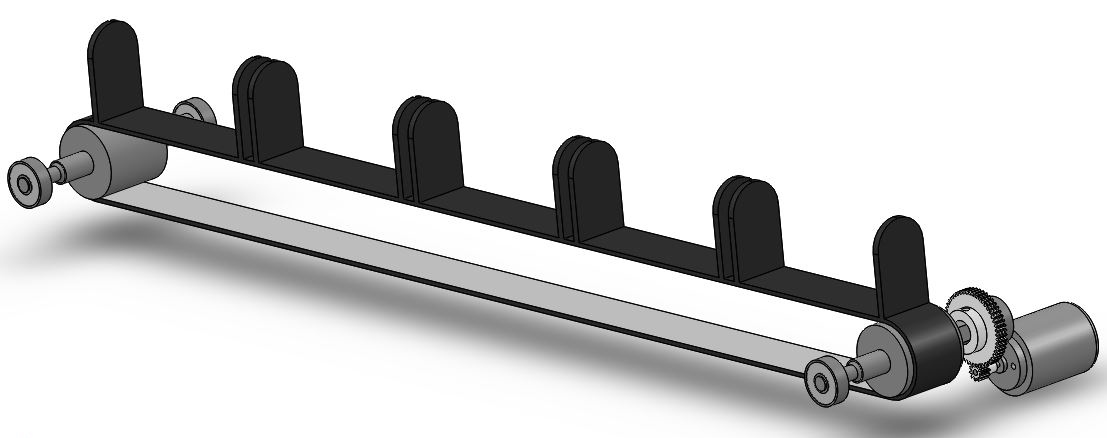
\includegraphics[width=0.9\textwidth,clip,trim=0mm 0mm 0mm 0mm]
    	{Enddokumentation/Bilder/Foerderband.jpg}
    	\centering
    	\caption{Aufbau des Förderbandes}
    	\label{abb:Foerderband}
 	\end{figure}

\subsection{Ansteuerung DC-Motor}
\label{sec:FoerderbandAnsteuerung}
    Die Ansteuerung des Motors, der das Förderband antreibt, erfolgt mittels PWM. Auf diese 
    Weise lässt sich die Drehzahl und somit die Nachführgeschwindigkeit einstellen. Das 
    Band muss nur in eine Richtung angetrieben werden, wodurch die Ansteuerung einfacher 
    realisiert werden kann. Das Schema ist in Abbildung \ref{abb:SchemaAnsteuerung} 
    ersichtlich. Im Wesentlichen besteht diese Ansteuerung aus einem Vortreiber und einem 
    Schalter. Der Treiber bewirkt ein möglichst schnelles und effizientes Öffnen und Schliessen des Schalters. Auf diese Weise reduziert man die Schaltverluste. 
    \begin{figure}[h!]
    	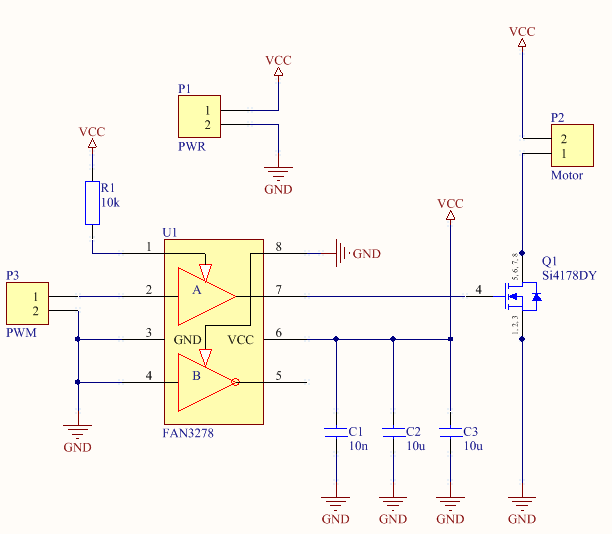
\includegraphics[width=0.7\textwidth,clip,trim=0mm 2mm 0mm 7mm]
    	{Enddokumentation/Bilder/Schema_DC-Ansteuerung.png}
    	\centering
    	\caption{Schema des Förderbandansteuerung}
    	\label{abb:SchemaAnsteuerung}
    \end{figure}